\documentclass{beamer}
\usepackage{graphicx}
\usepackage{xcolor}
\usepackage{tikz}
\usepackage{amsmath}
\usepackage{pgfplots}
\pgfplotsset{compat=1.18}

\definecolor{purpleblue}{RGB}{80, 80, 180}
\definecolor{novelPurple}{RGB}{98, 54, 255}
\definecolor{softPurple}{RGB}{180, 170, 255}
\definecolor{softGray}{RGB}{235, 235, 245}
\definecolor{lightText}{RGB}{90, 90, 110}

\usetheme{Madrid}
\usecolortheme{dolphin}
\graphicspath{{static/course_materials/}{static/hard/}{./}}

\setbeamerfont{title}{size=\Large,series=\bfseries}
\setbeamerfont{frametitle}{size=\LARGE,series=\bfseries}
\setbeamercolor{frametitle}{fg=white, bg=novelPurple}
\setbeamercolor{title}{fg=white, bg=purpleblue}

\title[Test VII]{\textbf{Test VII}}
\author{\textbf{Jack Zeng}}
\institute{\textcolor{white}{\textbf{Novel Prep}}}
\date{\today}

\begin{document}

\begin{frame}
    \titlepage
    \vfill
    \begin{flushright}
        \textcolor{purpleblue}{\Huge \textbf{Novel Prep}}
    \end{flushright}
\end{frame}

\begin{frame}
    \begin{tikzpicture}[remember picture, overlay]
        \shade[top color=softPurple, bottom color=softGray]
            (current page.north west) rectangle (current page.south east);
        \node[align=center] at (current page.center) {
            {\Huge\bfseries\textcolor{purpleblue}{Novel Prep}} \\[0.5cm]
            {\Large\itshape\textcolor{lightText}{Phase 3 · Mock Exam Training}}
        };
    \end{tikzpicture}
\end{frame}

\begin{frame}{Overview}
    \tableofcontents
\end{frame}

\begin{frame}
\section{Test VII}
    \begin{tikzpicture}[remember picture, overlay]
        \shade[top color=softPurple, bottom color=softGray]
            (current page.north west) rectangle (current page.south east);
        \node[align=center] at (current page.center) {
            {\LARGE\bfseries\textcolor{purpleblue}{Test VII}} \\[0.5cm]
            {\Large\itshape\textcolor{lightText}{22 easy-to-hard Module 2-style practice questions}}
        };
    \end{tikzpicture}
\end{frame}

% --- Question 1 ---
\begin{frame}{Question 1}
\small
A chemist mixed \(x\) liters of a \(6\%\) saline solution with \(y\) liters of a
\(9\%\) saline solution to produce a \(7\%\) saline solution. Which equation best
represents this situation? (Assume the volumes of the solutions are additive.)
\vspace{0.35cm}
\begin{enumerate}
    \item[A.] \(0.06x+0.09y=7(x+y)\)
    \item[B.] \(0.06x+0.09y=0.07(x+y)\)
    \item[C.] \(0.6x+0.9y=7(x+y)\)
    \item[D.] \(0.6x+0.9y=0.7(x+y)\)
\end{enumerate}
\end{frame}
\begin{frame}{Answer 1}
\small
\textbf{Correct Answer:} B
\end{frame}

% --- Question 2 ---
\begin{frame}{Question 2}
\small
A window repair specialist charges \(\$220\) for the first two hours of repair
plus an hourly fee for each additional hour. The total cost for \(5\) hours of
repair is \(\$400\). Which function \(f\) gives the total cost, in dollars, for
\(x\) hours of repair, where \(x\ge 2\)?
\vspace{0.35cm}
\begin{enumerate}
    \item[A.] \(f(x)=60x+100\)
    \item[B.] \(f(x)=60x+220\)
    \item[C.] \(f(x)=80x\)
    \item[D.] \(f(x)=80x+220\)
\end{enumerate}
\end{frame}
\begin{frame}{Answer 2}
\small
\textbf{Correct Answer:} A
\end{frame}

% --- Question 3 ---
\begin{frame}{Question 3}
\small
In the \(xy\)-plane, the graph of the linear function \(f\) has a negative slope
and a \(y\)-intercept at \((0,k)\), where \(k\) is a positive constant. Which of
the following must be true?
\[
\begin{array}{ll}
\text{I.} & \text{If }a>b,\text{ then }f(a)<f(b).\\
\text{II.} & \text{If }a<0,\text{ then }f(a)>k.\\
\text{III.} & \text{If }a>0,\text{ then }f(a)>0.
\end{array}
\]
\vspace{0.35cm}
\begin{enumerate}
    \item[A.] I and II only
    \item[B.] I and III only
    \item[C.] II and III only
    \item[D.] I, II, and III
\end{enumerate}
\end{frame}
\begin{frame}{Answer 3}
\small
\textbf{Correct Answer:} A
\end{frame}

% --- Question 4 ---
\begin{frame}{Question 4}
\small
In the given equation, \(k\) is a positive constant. What is the product of the
solutions to the given equation?
\[
x^2-8kx-(k-4)=0
\]
\vspace{0.35cm}
\begin{enumerate}
    \item[A.] \(4-k\)
    \item[B.] \(k-4\)
    \item[C.] \(-8k\)
    \item[D.] \(8k\)
\end{enumerate}
\end{frame}
\begin{frame}{Answer 4}
\small
\textbf{Correct Answer:} A
\end{frame}

% --- Question 5 ---
\begin{frame}{Question 5}
\small
The equation \(2|x-5|=k\), where \(k\) is a constant, has exactly one solution.
Which of the following could be the value of \(\frac{k}{2}\)?
\vspace{0.35cm}
\begin{enumerate}
    \item[A.] \(-5\) only
    \item[B.] \(-5\) or \(5\)
    \item[C.] \(0\) only
    \item[D.] \(5\) only
\end{enumerate}
\end{frame}
\begin{frame}{Answer 5}
\small
\textbf{Correct Answer:} C
\end{frame}

% --- Question 6 ---
\begin{frame}{Question 6}
\small
A manufacturer uses two assembly lines to produce refrigerator units. The table
summarizes the results of a quality-control test used to check for defective
units. If a refrigerator unit that was checked during this test is selected at
random, what is the probability that the unit was produced by assembly line A,
given that the unit is defective?
\[
\begin{array}{c|ccc}
&\text{Defective}&\text{Not defective}&\text{Total}\\ \hline
\text{Assembly line A}&300&5700&6000\\
\text{Assembly line B}&500&3500&4000\\ \hline
\text{Total}&800&9200&10000
\end{array}
\]
\vspace{0.35cm}
\begin{enumerate}
    \item[A.] \(\frac1{20}\)
    \item[B.] \(\frac38\)
    \item[C.] \(\frac35\)
    \item[D.] \(\frac58\)
\end{enumerate}
\end{frame}
\begin{frame}{Answer 6}
\small
\textbf{Correct Answer:} B
\end{frame}

% --- Question 7 ---
\begin{frame}{Question 7}
\small
A researcher wanted to determine whether studying at a library is more effective
than studying at home. He selected a random sample of \(200\) students and gave
them three days to study for the same test. The \(100\) students who lived closest
to a library were asked to study at a library, and the remaining \(100\) students
were asked to study at home. After the students took the test, the scores of those
who studied at a library were compared to the scores of those who studied at
home. How should this experiment be changed so that the researcher can conclude
whether studying at a library is more effective than studying at home?
\vspace{0.35cm}
\begin{enumerate}
    \item[A.] The students assigned to study at a library should study at the same library.
    \item[B.] The students should be randomly assigned to study either at a library or at home.
    \item[C.] The students assigned to study at a library should take a more difficult test than the students assigned to study at home.
    \item[D.] No changes to the experiment are necessary.
\end{enumerate}
\end{frame}
\begin{frame}{Answer 7}
\small
\textbf{Correct Answer:} B
\end{frame}

% --- Question 8 ---
\begin{frame}{Question 8}
\small
All the residents of a town were mailed a survey about proposed renovations to
the town's high school. Approximately \(10\%\) of the residents completed the
survey and mailed it back. Based on the responses, it was estimated that \(72\%\)
of the residents support the proposed renovations, with an associated margin of
error of \(12\%\). Which of the following best explains why these survey results
are unlikely to represent the opinions of all the town's residents?
\vspace{0.35cm}
\begin{enumerate}
    \item[A.] The survey included residents who do not attend the high school.
    \item[B.] Not all residents were aware of the proposed renovations before the survey.
    \item[C.] Responses to the survey were not obtained from a random sample of the town's residents.
    \item[D.] The margin of error is greater than the percentage of residents who responded to the survey.
\end{enumerate}
\end{frame}
\begin{frame}{Answer 8}
\small
\textbf{Correct Answer:} C
\end{frame}

% --- Question 9 ---
\begin{frame}{Question 9}
\small
The estimated total pressure a diver experiences below the surface of the water
is equal to the sum of the estimated water pressure and the estimated atmospheric
pressure. At a depth of \(h\) meters below the surface, the estimated total
pressure \(P_1\), in kilopascals (kPa), is given by
\[
P_1=10h+101.
\]
After maintaining a depth of \(h\) meters, the diver descended \(d\) additional
meters. The estimated total pressure \(P_2\), in kPa, after descending these
\(d\) additional meters is given by
\[
P_2=10d+341.
\]
What is the estimated total pressure, in kPa, the diver experienced at a depth
of \(h\) meters below the surface?
\vspace{0.35cm}
\begin{enumerate}
    \item[A.] 442
    \item[B.] 341
    \item[C.] 101
    \item[D.] 10
\end{enumerate}
\end{frame}
\begin{frame}{Answer 9}
\small
\textbf{Correct Answer:} B
\end{frame}

% --- Question 10 ---
\begin{frame}{Question 10}
\small
For each real number \(r\), which of the following points lies on the graph of
each equation in the \(xy\)-plane for the given system?
\[
\begin{aligned}
8x+7y&=9\\
24x+21y&=27
\end{aligned}
\]
\vspace{0.35cm}
\begin{enumerate}
    \item[A.] \(\left(r,\frac{-8r+9}{7}\right)\)
    \item[B.] \(\left(\frac{-8r+9}{7},r\right)\)
    \item[C.] \(\left(\frac{-8r+63}{7},\frac{9r+189}{7}\right)\)
    \item[D.] \(\left(\frac r3+9,-\frac r3+27\right)\)
\end{enumerate}
\end{frame}
\begin{frame}{Answer 10}
\small
\textbf{Correct Answer:} A
\end{frame}

% --- Question 11 ---
\begin{frame}{Question 11}
\small
An object's speed, in meters per hour, is increasing at a rate of \(1{,}490\)
meters per hour per second. Which of the following is closest to this rate in
feet per second squared? (Use \(1\) meter \(=3.28\) feet.)
\vspace{0.35cm}
\begin{enumerate}
    \item[A.] 0.126
    \item[B.] 1.36
    \item[C.] 7.57
    \item[D.] 81.5
\end{enumerate}
\end{frame}
\begin{frame}{Answer 11}
\small
\textbf{Correct Answer:} B
\end{frame}

% --- Question 12 ---
\begin{frame}{Question 12}
\small
In the given system of equations, \(b\) is a constant. If the system has no
solution, what is the value of \(b\)?
\[
\begin{aligned}
\frac3{10}y+\frac b3x&=\frac34-\frac15y\\
\frac38x+\frac35&=-\frac14y+\frac85
\end{aligned}
\]
\end{frame}
\begin{frame}{Answer 12}
\small
\textbf{Final Answer:} $\boxed{\dfrac{9}{4}}$
\end{frame}

% --- Question 13 ---
\begin{frame}{Question 13}
\small
A computer program models the population of a certain insect in an environment
where the insect has no natural predators. According to the model, the estimated
total mass of the population of insects at the end of every \(5\)-week period is
\(158\%\) greater than the estimated total mass at the end of the previous
\(5\)-week period. The estimated total mass at the end of \(15\) weeks is
\(627.7\) grams. Which equation best represents this model, where \(M\) is the
estimated total mass, in grams, at the end of \(t\) weeks?
\vspace{0.35cm}
\begin{enumerate}
    \item[A.] \(M=538.92(1.58)^{t/5}\)
    \item[B.] \(M=457.66(2.58)^{t/5}\)
    \item[C.] \(M=159.14(1.58)^{t/5}\)
    \item[D.] \(M=36.55(2.58)^{t/5}\)
\end{enumerate}
\end{frame}
\begin{frame}{Answer 13}
\small
\textbf{Correct Answer:} D
\end{frame}

% --- Question 14 ---
\begin{frame}{Question 14}
\small
Which expression is a factor of
\[
x^4+14ax^2+49a^2-64,
\]
where \(a\) is a positive constant?
\vspace{0.35cm}
\begin{enumerate}
    \item[A.] \(x^2+7a+8\)
    \item[B.] \(x^2-7a-8\)
    \item[C.] \(x^2+14a\)
    \item[D.] \(x^2-8a\)
\end{enumerate}
\end{frame}
\begin{frame}{Answer 14}
\small
\textbf{Correct Answer:} A
\end{frame}

% --- Question 15 ---
\begin{frame}{Question 15}
\small
The figure shown is a trirectangular tetrahedron, a three-dimensional figure
with four triangular faces, three of which are right triangles. The base is an
isosceles right triangle whose legs each have length \(12\) inches. The height
of the tetrahedron is \(24\) inches. Which of the following is closest to the
volume of this tetrahedron, in pints?

\begin{center}
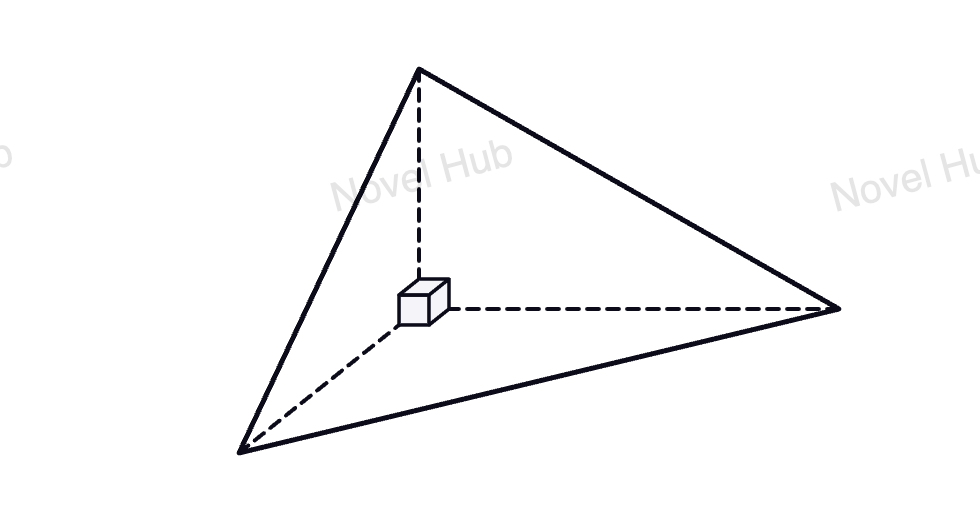
\includegraphics[width=0.5\linewidth]{hard_26_f15.png}

Note: Figure not drawn to scale.
\end{center}
\noindent Use \(1\) quart \(=57.75\text{ in}^3\), \(1\) pint \(=0.5\) quart, and
\(V=\frac13Sh\), where \(S\) is the area of the base and \(h\) is the height.
\vspace{0.35cm}
\begin{enumerate}
    \item[A.] 19.95
    \item[B.] 119.69
    \item[C.] 576.00
    \item[D.] 16,632.00
\end{enumerate}
\end{frame}
\begin{frame}{Answer 15}
\small
\textbf{Correct Answer:} A
\end{frame}

% --- Question 16 ---
\begin{frame}{Question 16}
\small
A right circular cone is inscribed in a sphere. The vertex of the cone is at the
top of the sphere, and the center of the cone's circular base is \(6\) inches
below the center of the sphere. The radius of the cone's base is \(8\) inches.
What is the volume, in cubic inches, of the cone?
\vspace{0.35cm}
\begin{enumerate}
    \item[A.] \(\frac{512\pi}{3}\)
    \item[B.] \(\frac{1024\pi}{3}\)
    \item[C.] \(384\pi\)
    \item[D.] \(\frac{1280\pi}{3}\)
\end{enumerate}
\end{frame}
\begin{frame}{Answer 16}
\small
\textbf{Correct Answer:} B
\end{frame}

% --- Question 17 ---
\begin{frame}{Question 17}
\small
In the given quadratic function, \(b\) and \(c\) are constants. The graph of
\(y=f(x)\) in the \(xy\)-plane does not intersect the \(x\)-axis. If
\(f(-7)=f(9)\), which of the following could be the value of \(b+c\)?
\[
f(x)=3x^2+bx+c
\]
\vspace{0.35cm}
\begin{enumerate}
    \item[A.] \(-1\)
    \item[B.] \(-3\)
    \item[C.] \(-5\)
    \item[D.] \(-7\)
\end{enumerate}
\end{frame}
\begin{frame}{Answer 17}
\small
\textbf{Correct Answer:} A
\end{frame}

% --- Question 18 ---
\begin{frame}{Question 18}
\small
In the given system of equations, \(p\) is a constant. The system has exactly one
distinct real solution \((x,y)\). What is the value of \(y\)?
\[
\begin{aligned}
y&=2x^2+15x+57\\
y&=-9x+p
\end{aligned}
\]
\end{frame}
\begin{frame}{Answer 18}
\small
\textbf{Final Answer:} $\boxed{39}$
\end{frame}

% --- Question 19 ---
\begin{frame}{Question 19}
\small
The graph of the quadratic function \(y=|a|x^2+bx+c\) passes through the
following five points:
\[
A(m,n),\quad B(0,y_1),\quad C(3-m,n),\quad
D(\sqrt2,y_2),\quad E(2,y_3).
\]
What is the correct order of \(y_1,y_2,y_3\)?
\vspace{0.35cm}
\begin{enumerate}
    \item[A.] \(y_1<y_2<y_3\)
    \item[B.] \(y_1<y_3<y_2\)
    \item[C.] \(y_3<y_2<y_1\)
    \item[D.] \(y_2<y_3<y_1\)
\end{enumerate}
\end{frame}
\begin{frame}{Answer 19}
\small
\textbf{Correct Answer:} D
\end{frame}

% --- Question 20 ---
\begin{frame}{Question 20}
\small
In rectangle \(ABCD\), point \(B\) is the center of a circle with radius \(BC\).
The circle intersects \(\overline{AB}\) at point \(F\). Point \(E\) lies on
\(\overline{AD}\), and segment \(CE\) is rotated about \(E\) to form \(EG\) such
that point \(G\) lies on the circle, where \(\angle GEC=90^\circ\). Point \(F\)
is the midpoint of \(\overline{EG}\). Given that \(AF=1\) and \(AE=3\), find the
length of \(CD\).

\begin{center}
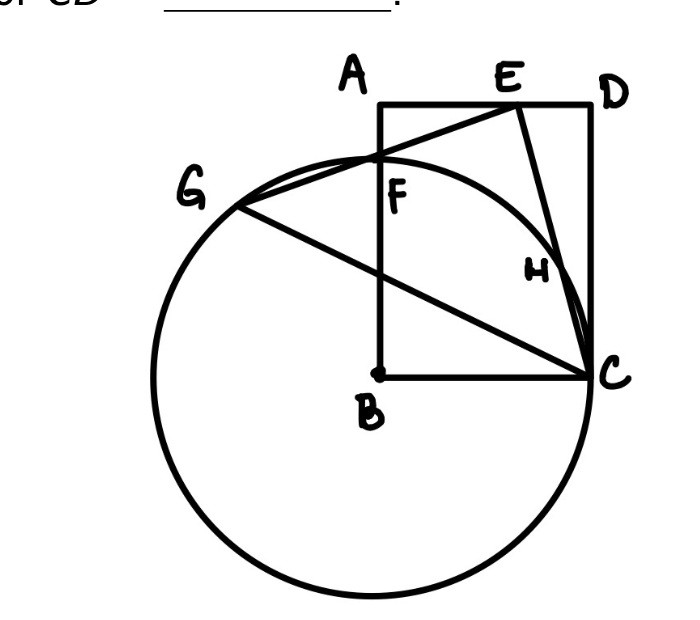
\includegraphics[width=0.5\linewidth]{hard_26_f20.png}
\end{center}
\end{frame}
\begin{frame}{Answer 20}
\small
\textbf{Final Answer:} $\boxed{6}$
\end{frame}

% --- Question 21 ---
\begin{frame}{Question 21}
\small
For what value of \(x\) is the given expression equivalent to
\((41k)^{25x}\), where \(k>1\)?
\[
\sqrt[8]{41k}\left(\sqrt[9]{41k}\right)^{12}
\]
\end{frame}
\begin{frame}{Answer 21}
\small
\textbf{Final Answer:} $\boxed{\dfrac{7}{120}}$
\end{frame}

% --- Question 22 ---
\begin{frame}{Question 22}
\small
In the given equation, \(p\) and \(w\) are integer constants. The equation has
exactly one real solution. Which is \textbf{NOT} a possible value of \(w\)?
\[
4x^2-px+w=-85
\]
\vspace{0.35cm}
\begin{enumerate}
    \item[A.] \(-21\)
    \item[B.] \(15\)
    \item[C.] \(64\)
    \item[D.] \(315\)
\end{enumerate}
\end{frame}
\begin{frame}{Answer 22}
\small
\textbf{Correct Answer:} C
\end{frame}

\begin{frame}{}
    \begin{tikzpicture}[remember picture, overlay]
        \shade[top color=novelPurple!40, bottom color=white]
            (current page.north west) rectangle (current page.south east);
        \fill[white, opacity=0.15] (current page.center) circle (5cm);
        \foreach \x in {1,2,3,4,5} {
            \fill[novelPurple, opacity=0.12] (rand*10-5, rand*7-3.5) circle (0.1+\x*0.05);
        }
    \end{tikzpicture}
    \centering
    \vspace{5em}
    {\Huge \textbf{\textcolor{novelPurple}{Thank You!}}} \\[1em]
    {\large \textcolor{gray}{We appreciate your time and focus.}} \\[3em]
    {\LARGE \textbf{\textcolor{novelPurple}{\textsf{Novel Prep}}}}
    \vfill
\end{frame}

\end{document}
